\documentclass[notes,11pt, aspectratio=169]{beamer}

\usepackage{pgfpages}
% These slides also contain speaker notes. You can print just the slides,
% just the notes, or both, depending on the setting below. Comment out the want
% you want.
\setbeameroption{hide notes} % Only slide
%\setbeameroption{show only notes} % Only notes
%\setbeameroption{show notes on second screen=right} % Both
\setbeamertemplate{caption}{\raggedright\insertcaption\par}


\usepackage{helvet}
\usepackage[default]{lato}
\usepackage{array}

\usepackage[backend=biber,style=authoryear,
sorting=ynt,citestyle=authoryear]{biblatex}
\addbibresource{Paper/papercitations.bib}

\usepackage{tikz}
\usepackage{verbatim}
\usepackage{animate}
\setbeamertemplate{note page}{\pagecolor{yellow!5}\insertnote}
\usetikzlibrary{positioning}
\usetikzlibrary{snakes}
\usetikzlibrary{calc}
\usetikzlibrary{arrows}
\usetikzlibrary{decorations.markings}
\usetikzlibrary{shapes.misc}
\usetikzlibrary{matrix,shapes,arrows,fit,tikzmark}
\usepackage{amsmath}
\usepackage{mathpazo}
\usepackage{hyperref}
\usepackage{lipsum}
\usepackage{multimedia}
\usepackage{graphicx}
\usepackage{multirow}
\usepackage{graphicx}
\usepackage{dcolumn}
\usepackage{bbm}
\newcolumntype{d}[0]{D{.}{.}{5}}
\usepackage{subfigure}
\usepackage{import}
\usepackage{fontawesome5}
\usepackage{subfig}
\usepackage{subcaption}

\usepackage[backend=biber,style=authoryear,
sorting=nyt,citestyle=authoryear]{biblatex}
\addbibresource{papercitations.bib}

\usepackage{changepage}
\usepackage{appendixnumberbeamer}
\newcommand{\beginbackup}{
   \newcounter{framenumbervorappendix}
   \setcounter{framenumbervorappendix}{\value{framenumber}}
   \setbeamertemplate{footline}
   {
     \leavevmode%
     \hline
     box{%
       \begin{beamercolorbox}[wd=\paperwidth,ht=2.25ex,dp=1ex,right]{footlinecolor}%
%         \insertframenumber  \hspace*{2ex} 
       \end{beamercolorbox}}%
     \vskip0pt%
   }
 }
\newcommand{\backupend}{
   \addtocounter{framenumbervorappendix}{-\value{framenumber}}
   \addtocounter{framenumber}{\value{framenumbervorappendix}} 
}

\setbeamertemplate{blocks}[rounded]
\setbeamercolor{block title}{bg=eggplant!70, fg=white}
\setbeamercolor{block body}{bg=eggplant!30}

\usepackage{graphicx}
\usepackage[space]{grffile}
\usepackage{booktabs}

% These are my colors -- there are many like them, but these ones are mine.
\definecolor{sage}{RGB}{102,153,102}
\definecolor{cambridgeblue}{RGB}{104, 166, 145}
\definecolor{yellow}{RGB}{255,173,1}
\definecolor{purple}{RGB}{153,102,153}
\definecolor{ashgray}{RGB}{191, 211, 193}
\definecolor{eggplant}{RGB}{105, 79, 93}
\definecolor{silver}{RGB}{192, 197, 193}
\definecolor{darkcyan}{RGB}{78, 135, 140}
\definecolor{lightcyan}{RGB}{201, 228, 231}
\definecolor{columbiablue}{RGB}{187, 213, 237}
\definecolor{lightblue}{RGB}{184, 219, 217}
\definecolor{earthyellow}{RGB}{234, 180, 100}

\setbeamercolor{mycolor}{fg=white,bg=sage}

% colors for diagrams
\definecolor{diagramtan}{RGB}{225,190,106}
\definecolor{diagramteal}{RGB}{64, 176, 166}
\definecolor{diagrampurple}{RGB}{170, 131, 239}
\definecolor{diagramred}{RGB}{146, 79, 79}


\hypersetup{
  colorlinks=false,
  linkbordercolor = {white},
  linkcolor = {sage}
}

\newcommand{\btVFill}{\vskip0pt plus 1filll}


%% I use a beige off white for my background
\definecolor{MyBackground}{RGB}{255,253,218}

%% Uncomment this if you want to change the background color to something else
%\setbeamercolor{background canvas}{bg=MyBackground}

%% Change the bg color to adjust your transition slide background color!
\newenvironment{transitionframe}{
  \setbeamercolor{background canvas}{bg=lightcyan}
  \begin{frame}[plain,noframenumbering]}{
    \end{frame}
}

\setbeamercolor{frametitle}{fg=black, bg=lightcyan}
\setbeamercolor{title}{fg=black}
\setbeamertemplate{footline}{%
  \raisebox{5pt}{\makebox[\paperwidth]{\hfill\makebox[15pt]{\scriptsize\insertframenumber}}}}
\setbeamertemplate{navigation symbols}{} 
\setbeamertemplate{itemize items}{$\bullet$}
\setbeamercolor{itemize item}{fg=lightcyan}
\setbeamercolor{itemize subitem}{fg=lightcyan}
\setbeamercolor{enumerate item}{fg=black}
\setbeamercolor{enumerate subitem}{fg=black}
\setbeamercolor{button}{bg=eggplant!80,fg=white}

\setbeamertemplate{frametitle}
{
    \nointerlineskip
    \begin{beamercolorbox}[sep=0.3cm,ht=2em,wd=\paperwidth]{frametitle}
        \vbox{}\vskip-2ex%
        \strut\insertframetitle\strut
        \vskip-0.8ex%
    \end{beamercolorbox}
}



% If you like road maps, rather than having clutter at the top, have a roadmap show up at the end of each section 
% (and after your introduction)
% Uncomment this is if you want the roadmap!
% \AtBeginSection[]
% {
%    \begin{frame}
%        \frametitle{Roadmap of Talk}
%        \tableofcontents[currentsection]
%    \end{frame}
% }

\setbeamercolor{section in toc}{fg=sage}
\setbeamercolor{subsection in toc}{fg=sage}
\setbeamersize{text margin left=1em,text margin right=1em} 

\newenvironment{wideitemize}{\itemize\addtolength{\itemsep}{10pt}}{\enditemize}

\usepackage{environ}
\NewEnviron{videoframe}[1]{
  \begin{frame}
    \vspace{-8pt}
    \begin{columns}[onlytextwidth, T] % align columns
      \begin{column}{.58\textwidth}
        \begin{minipage}[t][\textheight][t]
          {\dimexpr\textwidth}
          \vspace{8pt}
          \hspace{4pt} {\Large \sc \textcolor{blue}{#1}}
          \vspace{8pt}
          
          \BODY
        \end{minipage}
      \end{column}%
      \hfill%
      \begin{column}{.42\textwidth}
        \colorbox{green!20}{\begin{minipage}[t][1.2\textheight][t]
            {\dimexpr\textwidth}
            Face goes here
          \end{minipage}}
      \end{column}%
    \end{columns}
  \end{frame}
}

\title[]{\textcolor{sage}{Does Hospital Leadership Matter? \newline
Evidence from Pay-for-Performance}}

\author[]{Hanna Glenn}
\date{}


\begin{document}

%%% TIKZ STUFF
\tikzset{   
        every picture/.style={remember picture,baseline},
        every node/.style={anchor=base,align=center,outer sep=1.5pt},
        every path/.style={thick},
        }
\newcommand\marktopleft[1]{%
    \tikz[overlay,remember picture] 
        \node (marker-#1-a) at (-.3em,.3em) {};%
}
\newcommand\markbottomright[2]{%
    \tikz[overlay,remember picture] 
        \node (marker-#1-b) at (0em,0em) {};%
}
\tikzstyle{every picture}+=[remember picture] 
\tikzstyle{mybox} =[draw=black, very thick, rectangle, inner sep=10pt, inner ysep=20pt]
\tikzstyle{fancytitle} =[draw=black,fill=red, text=white]
%%%% END TIKZ STUFF

% Title Slide
\begin{frame}[plain]
% Background image
\begin{tikzpicture}[remember picture,overlay]
    \node
[
    above=0.5cm,
    align=center,
    fill=lightcyan,
    rounded corners,
    inner xsep=15pt,
    inner ysep=10pt, 
    minimum width=0.9\textwidth,
    text width=0.9\textwidth
] (title) at (current page.center)
{
    \LARGE Beyond Mergers: \\
    
    \vspace{3mm}
    \Large Informal Governance Ties and Hospital Behavior
};
% Author 
\node[below=1cm] (author) at (title.south){\large Hanna Glenn, The University of Queensland};
% Date
\node[below=0.25cm] (date) at (author.south){\today};
\end{tikzpicture}
    
\end{frame}

\section{Intro}

\large

\begin{frame}{General Increasing Consolidation in Hospital Markets}
    \begin{columns}
        \column{0.5\textwidth}
            \begin{figure}
                \centering
                \caption{Percent of HRRs with HHI $>$ 1,800}
                \includegraphics[width=\linewidth]{Objects/hhi_graph.pdf}
            \end{figure}

        \column{0.5\textwidth}
            \begin{wideitemize}
                \item Hospital markets are becoming increasingly concentrated
                \item 1,600 mergers from 1998 to 2017 \small (\cite{gaynor2020health}) \large
                \item This has led to increased scrutiny of mergers and acquisitions
            \end{wideitemize}
    \end{columns}
\end{frame}


\section{Hospital Consolidation Intro}

\begin{frame}[t]{What We Already Know}
\centering

\vspace{15mm}

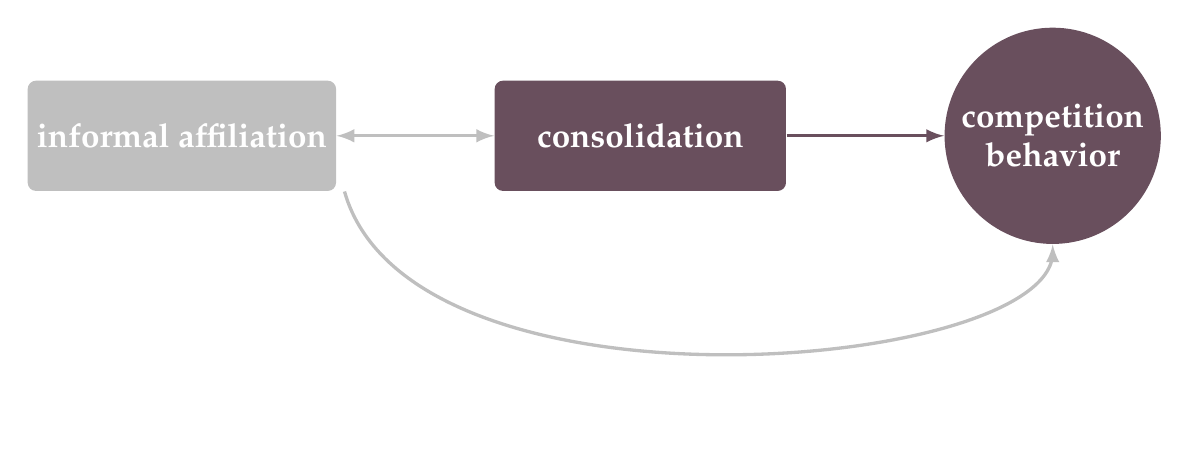
\begin{tikzpicture}[
    node distance=2cm,
    >=latex,
    % node styles
    box/.style = {
      draw=none,
      rounded corners=3pt,
      minimum width=3.7cm,
      minimum height=1.4cm,
      align=center,
      font=\bfseries\large,
      text=white
    },
    circ/.style = {
      circle,
      minimum size=2.4cm,
      align=center,
      font=\bfseries\large,
      text=white,
      draw=none
    },
    % arrow styles
    twoarr/.style = {<->, line width=1.2pt, draw=lightgray},
    arr/.style = {->, line width=1.2pt, draw=eggplant},
    underarr/.style= {->, line width=1.2pt, draw=lightgray}
  ]

  % --- Nodes
  \node[box, fill=lightgray] (affil) {informal affiliation};

  \node[box, fill=eggplant, right=of affil] (cons) {consolidation};

  \node[circ, fill=eggplant, right=of cons] (comp) {competition\\behavior};

  % --- Arrows
  \draw[twoarr] (affil) -- (cons);
  \draw[arr]  (cons) -- (comp);
    \path
    (affil.south east) ++(0.1cm,0) coordinate (startBelow);
  \path
    (comp.south) ++(0,-1.6cm) coordinate (midBelow); % how far down to dip
  \draw[underarr]
    (startBelow)
      .. controls ($(affil.south)!0.5!(cons.south) + (0,-3cm)$) and (midBelow) ..
    ($(comp.south) + (0,-0.1cm)$) -- (comp);
  

\end{tikzpicture}
\end{frame}


\begin{frame}{Hospital Consolidation Literature}
Operating costs/efficiency
\begin{itemize}
    \item Early studies found no effect \small \textcolor{lightgray}{(\cite{alexander1996short}; \cite{ho2000hospital})} \large
    \item More recent work does document increased efficiency \small \textcolor{lightgray}{(\cite{schmitt2017hospital}; \cite{andreyeva2024corporatization}; \cite{craig2021mergers})} \large
\end{itemize}

\vspace{1mm}

Price/quality
\begin{itemize}
    \item Consistently raised prices \small \textcolor{lightgray}{(\cite{gaynor2012impact}; \cite{boozary2019association}; \cite{cooper2019price}; \cite{andreyeva2024corporatization})} \large
    \item Mixed evidence on quality \small \textcolor{lightgray}{(\cite{haas2011mergers}; \cite{beaulieu2020changes}; \cite{hayford2012impact}; \cite{andreyeva2024corporatization})} \large
\end{itemize}

\vspace{1mm}

Other behaviors/mechanisms
    \begin{itemize}
        \item Convergence/changes in treatment styles \small \textcolor{lightgray}{(\cite{eliason2020acquisitions}; \cite{mariani2022impact})} \large
        \item Shifts in admission patterns \small \textcolor{lightgray}{(\cite{desai2023hospital})} \large
    \end{itemize}

    \vspace{2mm}

\textit{Effects are mitigated with more distance between the hospitals \small  (\cite{cooper2019price}) \large}

\end{frame}

\section{Informal Affiliation Intro}

\begin{frame}[t]{What We Know Less About}
\centering

\vspace{15mm}

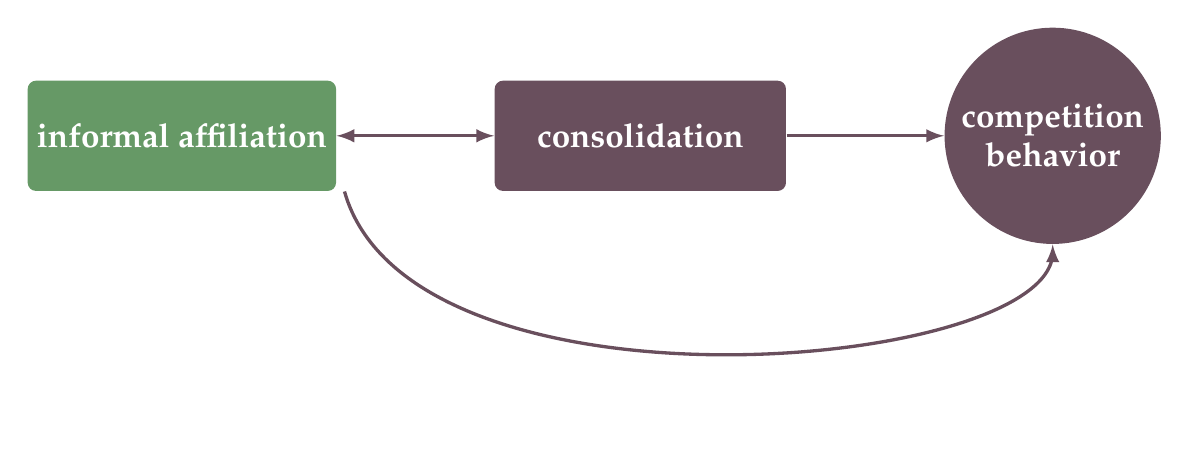
\begin{tikzpicture}[
    node distance=2cm,
    >=latex,
    % node styles
    box/.style = {
      draw=none,
      rounded corners=3pt,
      minimum width=3.7cm,
      minimum height=1.4cm,
      align=center,
      font=\bfseries\large,
      text=white
    },
    circ/.style = {
      circle,
      minimum size=2.4cm,
      align=center,
      font=\bfseries\large,
      text=white,
      draw=none
    },
    % arrow styles
    twoarr/.style = {<->, line width=1.2pt, draw=eggplant},
    arr/.style = {->, line width=1.2pt, draw=eggplant},
    underarr/.style= {->, line width=1.2pt, draw=eggplant}
  ]

  % --- Nodes
  \node[box, fill=sage] (affil) {informal affiliation};

  \node[box, fill=eggplant, right=of affil] (cons) {consolidation};

  \node[circ, fill=eggplant, right=of cons] (comp) {competition\\behavior};

  % --- Arrows
  \draw[twoarr] (affil) -- (cons);
  \draw[arr]  (cons) -- (comp);
    \path
    (affil.south east) ++(0.1cm,0) coordinate (startBelow);
  \path
    (comp.south) ++(0,-1.6cm) coordinate (midBelow); % how far down to dip
  \draw[underarr]
    (startBelow)
      .. controls ($(affil.south)!0.5!(cons.south) + (0,-3cm)$) and (midBelow) ..
    ($(comp.south) + (0,-0.1cm)$) -- (comp);
  

\end{tikzpicture}
\end{frame}

\begin{frame}{Unregulated Consolidation}
    While they don't commonly garner national attention, there are other hospital affiliations that could be important

    \vspace{10mm}

    \begin{columns}[T]
        \column{0.5\textwidth}
        \centering
        \textcolor{eggplant}{Small-scale Mergers}

        \vspace{3mm}

        \begin{wideitemize}
        \item ``Stealth mergers"
            \item Can reduce competition \\ \small \textcolor{lightgray}{(\cite{majerovitz2021consolidation}; \cite{aggarwal2025stealth}; \cite{wollmann2019stealth}; \cite{wollmann2020get}; \cite{kepler2023stealth})} \large
        \end{wideitemize}

        \column{0.5\textwidth}
        \centering
        \textcolor{eggplant}{Informal Affiliations}

        \vspace{3mm}

        \begin{wideitemize}
            \item Joint ventures; Clinical agreements; Shared members of leadership
            \item Several states have begun regulation these types of affiliations
        \end{wideitemize}
    \end{columns}
\end{frame}

\begin{frame}{Informal Affiliations: A Note of Transparency}
    In this paper, how I measure informal affiliation is strictly by \underline{overlapping leadership}

    \vspace{10mm}

    This is important and relevant on its own
    \begin{itemize}
        \item In the Clayton Act
        \item FTC has targeted it directly
    \end{itemize}

    \vspace{3mm}

    However, could be correlated with other types of affiliation
    \begin{itemize}
        \item There is no data to verify this
        \item I will investigate mechanisms to try to tease it out
    \end{itemize}

\end{frame}

\begin{frame}[t]{This Paper}
\centering

\vspace{8mm}

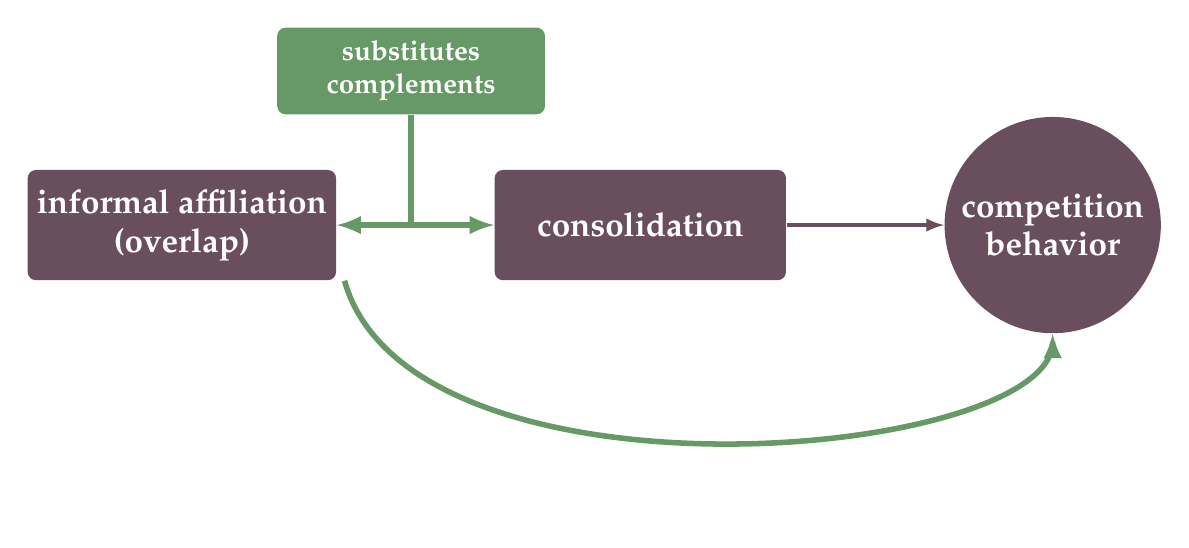
\begin{tikzpicture}[
    node distance=2cm,
    >=latex,
    % node styles
    box/.style = {
      draw=none,
      rounded corners=3pt,
      minimum width=3.7cm,
      minimum height=1.4cm,
      align=center,
      font=\bfseries\large,
      text=white
    },
    circ/.style = {
      circle,
      minimum size=2.4cm,
      align=center,
      font=\bfseries\large,
      text=white,
      draw=none
    },
    note/.style = {
      draw=none,
      rounded corners=3pt,
      minimum width=3.4cm,
      minimum height=1.1cm,
      align=center,
      font=\bfseries\normalsize,
      text=white,
      fill=sage
    },
    % arrow styles
    twoarr/.style = {<->, line width=2pt, draw=sage}, % same as <-> but explicit
    arr/.style = {->, line width=1.2pt, draw=eggplant},
    underarr/.style= {->, line width=2pt, draw=sage}
  ]

  % --- Nodes
  \node[box, fill=eggplant] (affil) {informal affiliation\\(overlap)};
  \node[box, fill=eggplant, right=of affil] (cons) {consolidation};
  \node[circ, fill=eggplant, right=of cons] (comp) {competition\\behavior};

  % --- Arrows
  \draw[twoarr] (affil) -- (cons);
  \draw[arr]  (cons) -- (comp);

  % Curved arrow under the nodes
  \path (affil.south east) ++(0.1cm,0) coordinate (startBelow);
  \path (comp.south) ++(0,-1.6cm) coordinate (midBelow); % how far down to dip
  \draw[underarr]
    (startBelow)
      .. controls ($(affil.south)!0.5!(cons.south) + (0,-3cm)$) and (midBelow) ..
    ($(comp.south) + (0,-0.1cm)$) -- (comp);

  % --- New "substitutes / complements" box above the middle of the affil<->cons arrow
  % Midpoint of the arrow between affil and cons
  \path let \p1 = ($(affil)!0.5!(cons)$) in coordinate (midAffCons) at (\x1,\y1);

  % The new box above that midpoint
  \node[note, above=1.4cm of midAffCons] (subs) {substitutes\\complements};

  % Arrow from the middle of the affil<->cons arrow up to the box
  \draw[-, line width=2pt, draw=sage] (midAffCons) -- (subs.south);
\end{tikzpicture}
\end{frame}

\section{Overlapping Leaders}

\begin{frame}{Overlapping Leaders: Does it Actually Happen?}
    \begin{columns}[T]
        \column{0.4\linewidth}
        \centering
        \includegraphics[width=0.9\textwidth]{clips/sevita_news.png}

        \column{0.6\linewidth}
        \centering
        \includegraphics[width=0.9\textwidth]{clips/affiliation1.png}

        \vspace{3mm}
        \includegraphics[width=0.9\textwidth]{clips/affiliation2.png}
    \end{columns}

    \vspace{5mm} \pause

\begin{itemize}
    \item Organizations denied merger permission b/c of it \small \textcolor{lightgray}{(\cite{huberfeld2006tackling})}\large, declaring informal affiliations through leadership \small \textcolor{lightgray}{(\cite{barnett_babcock_2012})}\large, and in life sciences companies \small \textcolor{lightgray}{(\cite{manjunath2024illegal})}\large
\end{itemize}
\end{frame}

\begin{frame}{Overlapping Leaders: Should it Actually Matter?}
    Board of Directors

    \vspace{2mm}
    \begin{wideitemize}
        \item Sets the broad direction of the firm and provides oversight
        \item Not in charge of day-to-day operations
    \end{wideitemize}

    \vspace{5mm}

    Board Governance is Correlated with Hospital Outcomes

    \vspace{2mm}
    \begin{wideitemize}
        \item Level of influence over the CEO \small (\cite{golden2001will}; \cite{alexander2008governance}; \cite{jiang2012enhancing}) \large
        \item Since the ACA, boards have been more directly involved in quality oversight \small (\cite{jha2010hospital}; \cite{prybil2010board}) \large
    \end{wideitemize}
\end{frame}

\section{Data}

\begin{transitionframe}
\centering
    \LARGE Documenting Leadership Overlap
\end{transitionframe}


\begin{frame}{Data on Boards/Executives}
\begin{itemize}
    \item Tax Forms 990s: Nonprofits
    \item 2013-2023
\end{itemize}

\vspace{5mm}

\begin{table}[ht!]
\centering
\begin{tabular}[t]{lcccccc}
\toprule
Sample & Num. People & Doctor & Nurse & Female & Connected & Connected\\
 & & & & & Same HRR & Diff. HRR\\
\midrule
\addlinespace[0.3em]
Board & 32,678 & 0.18 & 0.03 & 0.30 & 0.01 & 0.06\\
Executive & 19,344 & 0.14 & 0.03 & 0.38 & 0.01 & 0.07\\
\bottomrule
\end{tabular}
\end{table}
\large
    
\end{frame}

\begin{frame}{Documenting Overlap}
    \begin{figure}
        \centering
        \caption{Prevalence of Board/Executive Overlap}
        \includegraphics[width=0.8\linewidth]{Objects/connected_percent.pdf}
    \end{figure}
\end{frame}

% \begin{frame}{Hospital Connections Over Time}
% \centering
% \animategraphics[
%   autoplay,
%   loop,
%   width=0.8\linewidth
% ]{2}{Objects/frames_hosp_conn_gif/frame_}{01}{08}
% %   ^fps       ^prefix         ^first ^last
% \end{frame}

\begin{frame}{HRRs with Connected Hospitals Over Time}
\centering
\animategraphics[
  autoplay,
  loop,
  width=0.8\linewidth
]{2}{Objects/frames_hrr_conn_gif/frame_}{01}{08}
%   ^fps       ^prefix         ^first ^last
\end{frame}

% \begin{frame}{Hospital Characteristics}
% \normalsize
%     \begin{table}[ht!]
% \centering
% \begin{tabular}[t]{lcccccc}
% \toprule
% Sample of Hosp. & N & Num. Beds & General & In System & Academic & Num. Nurses\\
% \midrule
% \addlinespace[0.3em]
% \multicolumn{7}{l}{\textbf{Become Connected}}\\
% \hspace{1em}Same HRR & 338 & 198 & 0.91 & 0.53 & 0.52 & 316\\
% \hspace{1em}Different HRR & 388 & 147 & 0.94 & 0.51 & 0.39 & 226\\
% \addlinespace[0.3em]
% \multicolumn{7}{l}{\textbf{Lose Connection}}\\
% \hspace{1em}Same HRR & 83 & 273 & 0.85 & 0.50 & 0.64 & 549\\
% \hspace{1em}Different HRR & 333 & 182 & 0.92 & 0.56 & 0.49 & 285\\
% \addlinespace[0.3em]
% \multicolumn{7}{l}{\textbf{Always Connected}}\\
% \hspace{1em}Same HRR & 37 & 369 & 0.94 & 0.48 & 0.71 & 706\\
% \hspace{1em}Different HRR & 591 & 233 & 0.93 & 0.61 & 0.56 & 406\\
% \addlinespace
% Never Connected & 49 & 97 & 0.92 & 0.48 & 0.20 & 112\\
% \bottomrule
% \end{tabular}
% \end{table}
% \end{frame}




\section{Leadership Overlap and Consolidation}


\begin{transitionframe}
\centering
    \LARGE Leadership Overlap and Consolidation
\end{transitionframe}

\begin{frame}{Overlap and Mergers/Acquisitions}

\vspace{2mm}
\begin{columns}[T]
        \column{0.5\textwidth}
        \centering
        \underline{Substitutes}

        \vspace{3mm}

        \begin{wideitemize}
        \item If the cost of formal mergers/acquisitions increases, hospitals might substitute towards informal agreements
        \end{wideitemize}

        \column{0.5\textwidth}
        \centering
        \underline{Complements}

        \vspace{3mm}

        \begin{itemize}
            \item Overlap could lead to consolidation later on because of an established relationship
            \item Overlap could occur before consolidation to smooth the transition
        \end{itemize}
    \end{columns}

   
\end{frame}

\begin{frame}{Joining a System as a Function of Gaining/Losing Overlap}
    Let's first look at the correlation of timing with gaining or losing overlap

    \vspace{5mm}

    \begin{wideitemize}
        \item Stacked event study with four types of treatment:
        \begin{enumerate}
            \item Gain overlap in the same HRR
            \item Gain overlap in a different HRR
            \item Lose overlap in the same HRR
            \item Lose overlap in a different HRR
        \end{enumerate}
        \item Outcome is an indicator for whether the hospital is affiliated with a system (exists in HRR and out of HRR)
    \end{wideitemize}
\end{frame}

\begin{frame}{Joining System in Same HRR as a Function of Gaining/Losing Overlap}
    \begin{figure}
        \centering
        \includegraphics[width=0.75\linewidth]{Objects/any_formal_sameHRR.pdf}
    \end{figure}
\end{frame}

\begin{frame}{Joining System in Diff HRR as a Function of Gaining/Losing Overlap}
    \begin{figure}
        \centering
        \includegraphics[width=0.75\linewidth]{Objects/any_formal_diffHRR.pdf}
    \end{figure}
\end{frame}

\begin{frame}{What if Mergers Become More/Less Costly?}
    This really just tells us there is correlation in the timing of overlap, but not much more

    \vspace{3mm}

    Leveraging how ``aggressive" national merger regulation is as a shock to informal affiliation
    \begin{wideitemize}
        \item Since informal affiliations are not nationally regulated, this measure is exogenous to informal affiliations such as overlap
        \item If mergers become more regulated and informal affiliations go down, we know they are \textcolor{purple}{complements}
        \item If mergers become more regulated and informal affiliations go up, they are \textcolor{purple}{substitutes}
    \end{wideitemize}
\end{frame}

\begin{frame}{What if Mergers Become More/Less Costly?}
    \begin{block}{Measure of National ``Aggresiveness" towards Consolidation:}
    \vspace{2mm}
        $$MergerCost_t = \frac{\text{Number of Actions}_t}{\text{Number of Proposals}_t}$$
        \vspace{2mm}
    \end{block}

    \vspace{8mm}

    $$\text{Overlap}_{ht} = MergerCost_t + \alpha_h + \gamma_{HRR}$$
    $$\text{Overlap}_{ht} = MergerCost_{t-1} + \alpha_h + \gamma_{HRR}$$
\end{frame}

\begin{frame}{What if Mergers Become More/Less Costly?}
    \begin{table}[ht!]
\centering
\begin{tabular}[t]{l>{}c>{}cc>{}c}
\toprule
 & Same HRR & Diff HRR & Same HRR & Diff HRR\\
  & Mergers & Mergers & Overlap & Overlap\\
\midrule
\addlinespace
Merger Cost$_t$ & \textcolor[HTML]{2E8B57}{-5.36 (0.48)} & \textcolor[HTML]{2E8B57}{-6.81 (0.57)} & -0.73 (0.58) & \textcolor[HTML]{E69F00}{3.09 (0.9)}\\
\addlinespace
Merger Cost$_{t-1}$ & \textcolor[HTML]{2E8B57}{-4.88 (0.47)} & \textcolor[HTML]{2E8B57}{-6.06 (0.57)} & -0.23 (0.59) & \textcolor[HTML]{E69F00}{3.28 (0.91)}\\
\addlinespace
\bottomrule
\end{tabular}
\end{table}

\vspace{10mm}

\textcolor{purple}{$\implies$ Mergers and overlap have little relationship when considering consolidation in the same HRR, but they seem to be substitutes when considering different HRRs}
\end{frame}



% \begin{frame}{Closing as a Function of Gaining/Losing Overlap}
%     \begin{figure}
%         \centering
%         \includegraphics[width=0.8\linewidth]{Objects/closure.pdf}
%     \end{figure}
% \end{frame}

\section{Leadership Overlap and Competition}

\begin{transitionframe}
    \LARGE \centering
    Leadership Overlap and Competition
\end{transitionframe}

\begin{frame}{Outcomes: Informed by Consolidation Literature}
    Quality
    \begin{itemize}
        \item Star Ratings (HCAHPS)
    \end{itemize}

    \vspace{2mm}

    Financial Behavior
    \begin{itemize}
        \item Operating Costs (HCRIS)
        \item Investment in capital/land/IT (HCRIS)
    \end{itemize}

    \vspace{2mm}

    Patient Populations
    \begin{itemize}
        \item Total discharges (HCRIS)
        \item Percent Medicare/Medicaid/Private Insurance (HCRIS)
    \end{itemize}

    \vspace{2mm}

    Product Differentiation
    \begin{itemize}
        \item Total services offered (AHA)
        \item Concentration of services offered (measured by beds devoted to each service: AHA)
    \end{itemize}
\end{frame}

\begin{frame}{Estimation}
    Much like merging, gaining or losing affiliation is \underline{not random}

    \vspace{2mm}
    \begin{itemize}
        \item So, what can be done?
        \item I'll limit the control group to those who eventually gain/lose overlap in a \textit{different} HRR
        \item Based on pre-trends, these groups are similar \textcolor{red}{(link to appendix slide with the graphs of the different groups)}
    \end{itemize}
\end{frame}

\begin{frame}{Estimation}
    Staggered treatment: gaining or losing overlap in the \underline{same} HRR:

    $$Y_{it} = \alpha + \sum_{k \neq -1} \beta_k \cdot D_{i,t+k} + \gamma_i + \delta_t + \varepsilon_{it}$$

    \vspace{10mm} \pause

    Identifying Assumptions:

    \vspace{2mm}
    \begin{itemize}
        \item Parallel trends within the selected sample
        \item No spillover effects
        \item No other events correlated with gaining/losing same-HRR overlap
    \end{itemize}
\end{frame}

\begin{frame}{Overlap and Quality}
    \begin{columns}
    \column{0.5\linewidth}
    \begin{figure}
        \centering
        \includegraphics[width=0.9\linewidth]{Objects/overall_rating.pdf}
        \caption{Overall Hospital Rating}
    \end{figure}

    \column{0.5\linewidth}
    \begin{figure}
        \centering
        \includegraphics[width=0.9\linewidth]{Objects/summary_rating.pdf}
        \caption{Summary of Rating Categories}
    \end{figure}
\end{columns}
\end{frame}

\begin{frame}{Overlap and Quality}
    \begin{columns}
    \column{0.5\linewidth}
    \begin{figure}
        \centering
        \includegraphics[width=0.9\linewidth]{Objects/doc_communication.pdf}
        \caption{Doctor Communication Rating}
    \end{figure}

    \column{0.5\linewidth}
    \begin{figure}
        \centering
        \includegraphics[width=0.9\linewidth]{Objects/care_transition.pdf}
        \caption{Care Transition Rating}
    \end{figure}
\end{columns}
\end{frame}

\begin{frame}{Overlap and Financial Behavior}
\begin{columns}
    \column{0.5\linewidth}
    \begin{figure}
        \centering
        \includegraphics[width=0.9\linewidth]{Objects/any_purch.pdf}
        \caption{Building/Equipment Purchases}
    \end{figure}

    \column{0.5\linewidth}
    \begin{figure}
        \centering
        \includegraphics[width=0.9\linewidth]{Objects/tot_operating_exp.pdf}
        \caption{Total Operating Expenses}
    \end{figure}
\end{columns}
\end{frame}

\begin{frame}{Overlap and Patient Population}
\begin{columns}
    \column{0.5\linewidth}
    \begin{figure}
        \centering
        \includegraphics[width=0.9\linewidth]{Objects/tot_discharges.pdf}
        \caption{Total Discharges}
    \end{figure}
\end{columns}
\end{frame}

\begin{frame}{Overlap and Patient Population}
\begin{columns}
    \column{0.5\linewidth}
    \begin{figure}
        \centering
        \includegraphics[width=0.9\linewidth]{Objects/perc_mcare.pdf}
        \caption{Medicare Discharges}
    \end{figure}

    \column{0.5\linewidth}
    \begin{figure}
        \centering
        \includegraphics[width=0.9\linewidth]{Objects/perc_mcaid.pdf}
        \caption{Medicaid Discharges}
    \end{figure}
\end{columns}
\end{frame}

\begin{frame}{Overlap and Service Offerings}
\begin{columns}
    \column{0.5\linewidth}
    \begin{figure}
        \centering
        \includegraphics[width=0.9\linewidth]{Objects/bed_conc.pdf}
        \caption{Service Concentration}
    \end{figure}

    \column{0.5\linewidth}
    \begin{figure}
        \centering
        \includegraphics[width=0.9\linewidth]{Objects/num_services.pdf}
        \caption{Total Services}
    \end{figure}
\end{columns}
\end{frame}

\begin{frame}{Conclusion}
    \begin{block}{Why do we need this paper?}
        Hospital consolidation continues to rise, and it's important to know whether to devote resources to regulating even informal affiliations
    \end{block}

    \vspace{5mm}

    \begin{wideitemize}
        \item Formal consolidation and leadership overlap are largely unrelated when thinking about relationships within the same HRR
        \begin{itemize}
            \item However, they seem to be substitutes when considering relationships outside of the market
        \end{itemize}

        \item Are within-market informal affiliations anti-competitive?
        \begin{itemize}
            \item Quality improves through better care coordination
            \item More services offered
            \item No change in patient flows (in aggregate)
        \end{itemize}
        
        
    \end{wideitemize}
\end{frame}




\end{document}
